
\subsection{Alignment Options and Bounding Box Control}
\label{pgfplots:sec:align}

\subsubsection{Basic Alignment}
Alignment works with two main methods: a coordinate where the axis shall be drawn and an ``anchor'' inside of the axis which shall be drawn at this particular coordinate. This methodology is common for each \Tikz\ node -- and an axis is nothing but a (special) \Tikz\ node. The coordinate can be specified using the |at| key, while the anchor can be specified with the |anchor| key. In most cases, it is sufficient to provide only an anchor -- unless one needs more than one axis in the same picture environment.

\begin{pgfplotskey}{at=\marg{coordinate expression}}
Assigns a position for the complete axis image. This option works similarly to the |at|-option of |\node[at=|\marg{coordinate expression}|]|, see~\cite{tikz}. The common syntax is |at={|\parg{x,y}|}|.

The idea is to provide an \meta{coordinate expression} where the axis will be placed. The axis' anchor will be placed at \meta{coordinate expression}.
\end{pgfplotskey}

\begin{pgfplotskey}{anchor=\marg{name} (initially south west)}
\label{option:anchor}%
Chooses one of the different possible positions inside of an axis which is placed with |at|. The |at| key defines the position where to place the axis inside of the embedding picture, the |anchor| key defines which point of the axis shall be positioned by `|at|'. The initial configuration assumes |at={(0,0)}|. Thus, |anchor=center| will place the axis' center at the logical picture position $(0,0)$. Similarly, |anchor=south west| will position the lower left corner of the axis at $(0,0)$.

For users who are familiar with \Tikz: an axis is actually a very special node, so anchors work as in~\cite{tikz}.

Anchors are useful in conjunction with horizontal or vertical alignment of plots, see the examples below.

There are four sets of anchors available: anchors positioned on the axis bounding box, anchors on the outer bounding box and anchors which have one coordinate on the outer bounding box and the other one at a position of the axis rectangle. Finally, one can place anchors near the origin.

{%
%\pgfplotsset{every picture/.append style={background rectangle/.style={help lines},show background rectangle}}%
\pgfplotstableread{pgfplots.testplot}\plottable
\def\plot{%
	\begin{axis}[
		width=5cm,
		name=test plot,
		xlabel=$x$,
		ylabel={$y$},% = \frac 12 \cdot x^3 - 4 x^2 -16 x$},
		legend style={at={(1.03,1)},anchor=north west},
		title=A test plot.
	]
		\addplot table from{\plottable};
		%\addplot coordinates {(0,0) (1,1)};
		\addlegendentry{$f(x)$}
		\addplot[red] plot[id=gnuplot_ppp,domain=-40:40,samples=120] gnuplot{10000*sin(x/3)};
		\addlegendentry{$g(x)$}
	\end{axis}
}%
\def\showit#1#2{%
	%\node[show them,#2] at (test plot.#1) {(s.#1)};
	\node[pin=#2:(s.#1),fill=black,circle,scale=0.3] at (test plot.#1) {};
}%
\tikzstyle{every pin}=[opacity=0.5,fill=yellow,rectangle,rounded corners=3pt,font=\tiny]%
In more detail, we have anchors on the axis rectangle (the bounding box around the axis)\footnote{Versions prior to \PGFPlots\ v.1.3 did \emph{not} use the bounding box of the axis, they used axis coordinates to orient these anchors. This has been fixed. If you \emph{really} want to undo the bugfix, see \texttt{\protect\pgfmanualpdfref{compat/anchors}{compat/anchors}}.},
		\begin{center}
			\begin{tikzpicture}
				\plot
				\showit{north}{90}
				\showit{north west}{135}
				\showit{west}{180}
				\showit{south west}{225}
				\showit{south}{270}
				\showit{south east}{305}
				\showit{east}{0}
				\showit{north east}{45}
				\showit{center}{90}
			\end{tikzpicture}
		\end{center}
Anchors on the outer bounding box,
		\begin{center}
			\begin{tikzpicture}
				\plot
				\showit{outer north}{90}
				\showit{outer north west}{135}
				\showit{outer west}{180}
				\showit{outer south west}{225}
				\showit{outer south}{270}
				\showit{outer south east}{305}
				\showit{outer east}{0}
				\showit{outer north east}{45}
				\showit{outer center}{90}
			\end{tikzpicture}
		\end{center}
There are anchors which have one coordinate on the outer bounding box, and one on the axis rectangle,
		\begin{center}
			\begin{tikzpicture}
				\plot
				{\pgfplotsset{every pin/.append style={pin distance=1cm}}%
				\showit{above north}{90}
				}%
				\showit{above north east}{45}
				\showit{right of north east}{0}
				\showit{right of east}{0}
				\showit{right of south east}{0}
				\showit{below south east}{-45}
				{\pgfplotsset{every pin/.append style={pin distance=1cm}}%
				\showit{below south}{-90}
				}%
				\showit{below south west}{-135}
				\showit{left of south west}{180}
				\showit{left of west}{180}
				\showit{left of north west}{180}
				\showit{above north west}{135}
			\end{tikzpicture}
		\end{center}
And finally, we have origin anchors which are especially useful when axis lines pass through the origin,
		\begin{center}
			\begin{tikzpicture}
					\begin{axis}[
						name=test plot,
						axis x line=center,
						axis y line=center,
						enlargelimits=false,
						minor tick num=3,
						tick style={semithick},
						tick align=center,
						xlabel=$x$,
						ylabel=$y$,
						every axis x label/.style={at={(current axis.right of origin)},anchor=north east},
						every axis y label/.style={at={(current axis.above origin)},anchor=north east},
						inner axis line style={->},
					]
					\addplot+[domain=-2:5] {20*x};
					\end{axis}
				{\pgfplotsset{every pin/.append style={pin distance=1cm}}%
				\showit{above origin}{45}
				}%
				\showit{right of origin}{45}
				{\pgfplotsset{every pin/.append style={pin distance=1cm}}%
				\showit{below origin}{0}
				}%
				\showit{left of origin}{135}
				\showit{origin}{135}
			\end{tikzpicture}
		\end{center}

		\noindent There is a fifth anchor which is not directly related to the axis: you can provide the anchor of \emph{a named inner node}. Thus, you can define your own anchor, by writing |\node (|\meta{name}|) at |\parg{point coordinate}| {};| as follows (using the |baseline| option described below):
\begin{codeexample}[]
Aligning at .......
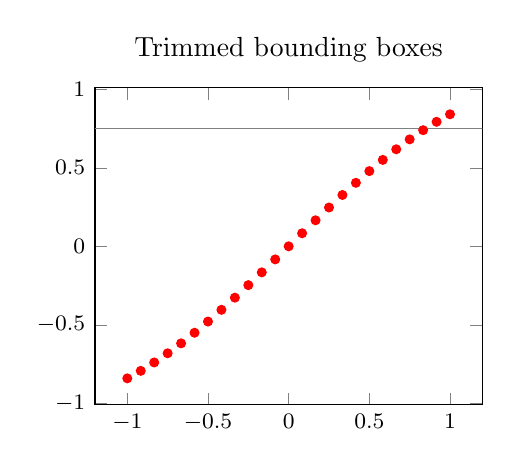
\begin{tikzpicture}[baseline]
\begin{axis}[small,anchor=aninnernode.center]
	\addplot {sin(deg(x))};
	\node
		[pin=-90:(aninnernode),fill=black,circle,scale=0.3] 
		(aninnernode) at (axis cs:-2,0.75) {};
	\draw[help lines] (axis cs:-6,0.75) -- (axis cs:6,0.75);
\end{axis}
\end{tikzpicture}
\end{codeexample}
\noindent What happens is that a node is placed at |(axis cs:-2,0.75)|. Note that the options |[pin=...]| are merely to show the |\node| (the pin style has been defined by the \PGFPlots\ manual). Since a name can also be assigned using |name=|\meta{node's name} and since any \PGFPlots\ description is also a |\node|, you can align your plot at selected axis descriptions:
\begin{codeexample}[]
Aligning at .......
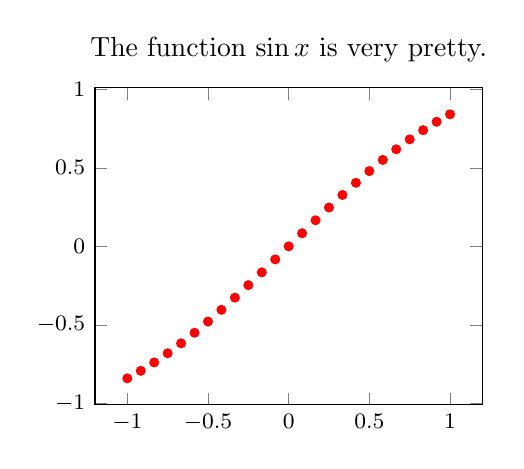
\begin{tikzpicture}[baseline]
\begin{axis}[
	small,
	title={The function $\sin x$ is very pretty.},
	title style={name=MyTitleNode},
	anchor=MyTitleNode.base,
]
	\addplot {sin(deg(x))};
\end{axis}
\end{tikzpicture}
\end{codeexample}

The default value is |anchor=south west|. 
You can use anchors in conjunction with the \Tikz\ |baseline| option and/or |\begin{pgfinterruptboundingbox}| to perform alignment.

\paragraph{Remarks:} Each of the anchors on the axis rectangle has an equivalent to a coordinate in the |axis description cs| described in Section~\ref{pgfplots:sec:axis:description:cs}. That means the first set of anchors actually lives on the \emph{tight bounding box around the axis} (without any ticks or descriptions). The |south west| anchor will always be the lower left corner of this bounding box, even in case of a rotated or skewed coordinate system\footnote{Note that this is only true for versions since 1.3.}. Similar statements hold for the other anchors.
}

\subsubsection{Vertical Alignment with \texttt{baseline}}
\label{sec:align}%
\begin{key}{/tikz/baseline}
The |baseline| option should be provided as argument to a |tikzpicture|. It configures \Tikz\ to shift the picture position $y=0$ to the embedding text's baseline:
\begin{codeexample}[width=3cm]
This is \tikz[baseline]\fill[red] (0,0) circle(3pt); a picture, 
here \tikz[baseline]\fill[red] (0,10pt) circle(3pt); another one.
\end{codeexample}
\noindent Consequently, the |baseline| option allows to align different |tikzpicture|s. An axis is, by default, placed with |at={(0,0)}|, and the |anchor| key specifies which part of the axis is placed at |(0,0)|. Consequently, the |baseline| option, together with |anchor|, allows to align different axes with the embedding text.

The default axis anchor is |south west|, which means that the picture coordinate $(0,0)$ is the lower left corner of the axis. As a consequence, the \Tikz\ option ``|baseline|'' allows vertical alignment of adjacent plots:
\begin{codeexample}[]
% 1. Unaligned:
\pgfplotsset{domain=-1:1}
\begin{tikzpicture}
	\begin{axis}[xlabel=A normal sized $x$ label]
	\addplot[smooth,blue,mark=*] {x^2};
	\end{axis}
\end{tikzpicture}%
\hspace{0.15cm}
\begin{tikzpicture}
	\begin{axis}[xlabel={$\displaystyle \sum_{i=0}^N n_i $ }]
	\addplot[smooth,blue,mark=*] {x^2};
	\end{axis}
\end{tikzpicture}
\end{codeexample}

\begin{codeexample}[]
% 2. Aligned:
\pgfplotsset{domain=-1:1}
\begin{tikzpicture}[baseline]
	\begin{axis}[xlabel=A normal sized $x$ label]
	\addplot[smooth,blue,mark=*] {x^2};
	\end{axis}
\end{tikzpicture}%
\hspace{0.15cm}
\begin{tikzpicture}[baseline]
	\begin{axis}[xlabel={$\displaystyle \sum_{i=0}^N n_i $ }]
	\addplot[smooth,blue,mark=*] {x^2};
	\end{axis}
\end{tikzpicture}
\end{codeexample}

	Note that it is also possible to write |baseline=5cm| in which case the image offset at $y=$|5cm| will be used as baseline.
\end{key}
The |baseline| key is related to |\begin{minipage}|\oarg{alignment} or |\begin{tabular}|\oarg{alignment}: the \meta{alignment} tells \LaTeX\ which part of the |minipage| or |tabular| shall be positioned on the baseline. Thus, |baseline| does the same for pictures (with more freedom for \meta{alignment}).

\subsubsection{Horizontal Alignment}
\label{sec:halign}%
Horizontal alignment can be done in two ways:
\begin{enumerate}
	\item Using separate |tikzpicture| environments which have reduced bounding boxes or
	\item A single |tikzpicture| environment in which the complete alignment is done.
\end{enumerate}
The first approach requires the use of reduced bounding boxes and is discussed in Section~\ref{sec:bb}.

The second approach, a single |tikzpicture| environment, employs the |at| and |anchor| keys to align parts of the images. For example, if you place multiple |axes| into a single |tikzpicture| and use the `|anchor|'-option, you can control horizontal alignment:
\begin{codeexample}[]
\begin{tikzpicture}
\pgfplotsset{every axis/.append style={
cycle list={
	{red,only marks,mark options={
		fill=red,scale=0.8},mark=*},
	{black,only marks,mark options={
		fill=black,scale=0.8},mark=square*}}}}

\begin{axis}[width=4cm,scale only axis,
	name=main plot]
\addplot file 
	{plotdata/pgfplots_scatterdata1.dat};
\addplot file 
	{plotdata/pgfplots_scatterdata2.dat};
\addplot[blue] coordinates {
	(0.093947,	-0.011481)
	(0.101957,	0.494273)
	(0.109967,	1.000027)};
\end{axis}

\begin{axis}[
	at={(main plot.below south west)},yshift=-0.1cm,
	anchor=north west,
	width=4cm,scale only axis,height=0.8cm,
	ytick=\empty]

\addplot file 
  {plotdata/pgfplots_scatterdata1_latent.dat};
\addplot file 
  {plotdata/pgfplots_scatterdata2_latent.dat};
\end{axis}
\end{tikzpicture}
\end{codeexample}

Here, the second axis uses |at={(main plot.below south west)}| to be placed below the first one. Furthermore, it has |yshift=-0.1cm| in order to leave additional space, and it uses |anchor=north west| to place the upper left corner at the specified position. Instead of the |at={}| construction, we could also have used |yshift| with larger negative shift.

\subsubsection{Alignment In Array Form (Subplots)}
\label{sec:pgfplots:arrayform}
\index{Subplots}%
\index{Alignment!Subplots}%
\index{Alignment!Array}%
\index{array!Array Alignment}%
\pgfmanualpdflabel{\textbackslash matrix}{}%
Sometimes multiple alignment axes in array form are desired. \PGFPlots\ supports this task in several ways which are described in the following. There are basically three related, yet different, approaches:
\begin{enumerate}
	\item Simply place |\begin{tikzpicture}...\end{tikzpicture}| into a \LaTeX\ table.
	This is straight--forward; you would do the very same thing with |\includegraphics|. 

	In addition to |\includegraphics|, the |baseline| feature allows simple yet effective vertical alignment. In addition, the |trim left| and |trim right| features allow simple yet effective horizontal alignment (see below).

	\item Use a \emph{single} picture which contains an array of axes, i.e.\ a pattern like

	|\begin{tikzpicture} \matrix{ |\meta{multiple axes}|}; \end{tikzpicture}|.

	This allows considerably simpler alignment! Alas, it needs special handling for |legend entries| due to a weakness of |\matrix|. If you use the |external| library (which is recommended), it takes more time since the picture gets larger.

	\item Use the |groupplots| library shipped with \PGFPlots. It is specialized on axes in array form with particular strength if the axes are closely related (for example if they share axis descriptions like |xlabel| or even tick labels). Note, however, that the other approaches are better when it comes to automatic handling of bounding boxes.
\end{enumerate}
The |groupplots| library is discussed in all detail in Section~\ref{sec:group:plot}. This section discusses the other two approaches.


\paragraph{Array Alignment using \LaTeX\ Tables}
The idea is simple: use a \LaTeX\ table and provide one |tikzpicture| for every cell. You are probably familiar with this sort of alignment, perhaps together with |\includegraphics|. It works in the very same way for \PGFPlots. The approach is the simplest one since it doesn't need special knowledge. Its disadvantage, however, is more difficulty to control positions \emph{inside} of the image (like differently sized axis descriptions).

Is is strongly recommended to employ the |baseline| option for each cell picture, which simplifies vertical alignment considerably. If you want a simple solution to place separate axes in array form, and you prefer to use one |tikzpicture| for every axis, the probably most simple and most effective way to get horizontal alignment are the |trim left| and |trim right| features -- or styles based on them:

The |trim axis left| feature can be used to exclude axis descriptions on the left from the bounding box, and the |trim axis right| can exclude axis descriptions on the right from the bounding box. Thus, alignment is done using the vertical axis lines. Since both keys effectively modify the bounding box, they are documented in Section~\ref{sec:bb} ``Bounding Box Restrictions''. Here is just a small example for array alignment by means of |tabular|, |baseline| and the |trim left|/|trim right| features:

\begin{codeexample}[vbox]
\pgfplotsset{
	small,
	title=Trimmed bounding boxes
}
\begin{center}
\begin{tabular}{rl}
	\begin{tikzpicture}[baseline,trim axis left]
		\begin{axis}
			\addplot {x};
		\end{axis}
	\end{tikzpicture}
	&
	\begin{tikzpicture}[baseline,trim axis right]
	\begin{axis}[
		ylabel={$f(x)=x^2$},
		yticklabel pos=right,
		ylabel style={font=\Huge}]
		\addplot {x^2};
	\end{axis}
	\end{tikzpicture}
	\\
	%
	\begin{tikzpicture}[baseline,trim axis left]
	\begin{axis}[xlabel=$x$,xlabel style={font=\Huge}]
		\addplot {x^3};
	\end{axis}
	\end{tikzpicture}%
	&
	\begin{tikzpicture}[baseline,trim axis right]
	\begin{axis}[yticklabel pos=right]
		\addplot {x^4};
	\end{axis}
	\end{tikzpicture}%
	\\
\end{tabular}%
\end{center}
\end{codeexample}
\noindent The example has $2 \times 2$ axes. The |baseline| feature controls the vertical alignment: the lower axis lines are always on the same height. The |trim axis left| key is a style which tells \Tikz\ to trim everything which is left of the left axis line. Similarly, the |trim axis right| key does not include picture parts right of the right axis line. Together with |\begin{center}| and the |yticklabel pos=right| key, we get correct horizontal and vertical alignment together with centering at the left- and right axis lines (without descriptions).

A strong advantage is that this type of alignment requires almost no changes to your pictures. Thus, you can copy--paste existing images (\TeX\ code) relatively simple.

Note that the approach is fully compatible with the image |external|ization library: each picture is exported separately, and the bounding box restrictions (and the |baseline| offset) are stored in separate |.dpth| files. The |trim left|/|trim right| approach for horizontal alignment is the \emph{only} supported way for reduced bounding boxes and image externalization.


\paragraph{Array Alignment using \Tikz\ Matrices}
While it is possible to use (for example) |tabular| combined with the vertical and horizontal alignment methods discussed above, it might be better to use a \Tikz\ |matrix| since it automatically handles the size of axis descriptions.

A \Tikz\ matrix is some sort of ``graphical'' table. It knows everything about picture alignment and it has more flexibility than |tabular| when it comes to graphics. The idea is to pack the complete array into a \emph{single} picture.

The complete documentation of a \Tikz\ matrix is beyond the scope of this manual, please refer to \cite{tikz} for details. But we provide an example here:
\pgfmanualpdflabel{/tikz/matrix}{}%
\begin{codeexample}[]
\begin{tikzpicture}
	\pgfplotsset{small}
	\matrix {
		\begin{axis}
			\addplot {x};
		\end{axis}
		&
		% differently large labels are aligned automatically:
		\begin{axis}[ylabel={$f(x)=x^2$},ylabel style={font=\Huge}]
			\addplot {x^2};
		\end{axis}
		\\
		%
		\begin{axis}[xlabel=$x$,xlabel style={font=\Huge}]
			\addplot {x^3};
		\end{axis}
		&
		\begin{axis}
			\addplot {x^4};
		\end{axis}
		\\
	};
\end{tikzpicture}
\end{codeexample}
\noindent So, a matrix is a picture element inside of |tikzpicture|. Its cells are separated by `|&|' as in tabular (or, if `|&|' causes problems, with |\pgfmatrixnextcell|). Its rows are separated by `|\\|'. Each cell is aligned using the cells' anchor. Since, by default, the anchor of an axis is placed at the lower left corner, the example above is completely aligned, without the need for any bounding box modifications -- even the labels are aligned correctly. If another anchor shall be used, simply place 
\begin{codeexample}[code only]
\pgfplotsset{anchor=....}
\matrix {
  ...
};
\end{codeexample}
\noindent in front of the matrix. This will use the same configuration for every sub-plot.

\paragraph{Attention:} Unfortunately, the array alignment with |\matrix| needs special \emph{attention with legends}. A legend is also a |\matrix| and \Tikz\ matrices can't be nested. You will need to use the |legend to name| feature (or to assemble a legend by means of |\label| and |\ref|) to overcome this weakness (see Section~\ref{pgfplots:legend:labelref} for details). 


\subsubsection{Miscellaneous for Alignment}

\begin{predefinednode}{current axis}
	A node which refers to the current axis or the last typeset axis.

	You can use this node in axis descriptions, for example to place axis labels or titles.

	\paragraph{Remark:} If you use |current axis| inside of axis descriptions, the ``current axis'' is not yet finished. That means you \emph{can't use any outer anchor} inside of axis descriptions.

	It is also possible to use |current axis| in any drawing or plotting commands inside of an axis (but no outer anchor as these are not defined when drawing commands are processed). This usage is similar to the |axis description cs|.
\end{predefinednode}

\subsubsection{Bounding box restrictions}
\label{sec:bb}
Bounding box restrictions can be archieved with several methods of \PGF:
\begin{enumerate}
	\item The |overlay| option,
	\item The |pgfinterruptboundingbox| environment,
	\item The |\pgfresetboundingbox| command,
	\item The |\useasboundingbox| path,
	\item The |trim left| and |trim right| feature (which is the \emph{only} supported way of restricted bounding boxes and image externalization; at least for \textsc{pdf} output). 
\end{enumerate}
Note that image externalization (the |external| library) is more or less incompatible with methods (1.)--(4.). The problem is that |pdflatex| crops everything outside of the bounding box away. There are only two safe ways to ``restrict'' bounding boxes of external |.pdf| images: the first is the mentioned |trim left|/|trim right| feature and the second is to use negative |\hspace| or |\vspace| commands (or options to |\includegraphics|).

\begin{key}{/tikz/overlay}
\index{Bounding Box Control!Excluding Image Parts}
	A special key of \PGF\ which disables bounding box updates for (parts of) the image. The effect is that those parts are an ``overlay'' over the document.

	For \PGFPlots, |overlay| can be useful to position legends or other axis descriptions outside of the axis~-- without affecting its size (and without affecting alignment).

For example, one may want to include only certain parts of the axis into the final bounding box. This would allow horizontal alignment (centering):
\begin{codeexample}[]
\begin{tikzpicture}%
   \begin{axis}[
      title=A title,
      ylabel style={overlay},
      yticklabel style={overlay},
      xlabel={$x$},
      ylabel={$y$},
      legend style={at={(0.5,0.97)},
         anchor=north,legend columns=-1},
      domain=-2:2
   ]
   \addplot {x^2};
   \addplot {x^3};
   \addplot {x^4};
   \legend{$x^2$,$x^3$,$x^4$}
   \end{axis}
\end{tikzpicture}%
\end{codeexample}
\noindent Now, the left axis descriptions ($y$ label and $y$ ticks) stick out of the bounding box.
	
The following example places a legend somewhere without affecting the bounding box.
\begin{codeexample}[]
\begin{tikzpicture}
   \begin{axis}[
      domain=0:6.2832,samples=200,
      legend style={
         overlay,
         at={(-0.5,0.5)},
         anchor=center},
      every axis plot post/.append style={mark=none},
      enlargelimits=false]

   \addplot {sin(deg(x)+3)+rand*0.05};
   \addplot {cos(deg(x)+2)+rand*0.05};
   \legend{Signal 1,Signal 2}
   \end{axis}
\end{tikzpicture}
\end{codeexample}

	More information about the |overlay| option can be found in the \PGF\ manual~\cite{tikz}.
\end{key}

\begin{command}{\pgfresetboundingbox}
	This command of \pgfname\ resets the bounding box of the current picture. The computation starts from scratch afterwards, allowing to compute a user--defined bounding box.
	
\begin{codeexample}[]
\setlength{\fboxsep}{0pt}%
\fbox{%
\begin{tikzpicture}%
	\begin{axis}[
		title=A title,
		xlabel={$x$},
		ylabel={$y$},
		legend style={at={(0.5,0.97)},
			anchor=north,legend columns=-1},
		domain=-2:2
	]
	\addplot {x^2};
	\addplot {x^3};
	\addplot {x^4};
	\legend{$x^2$,$x^3$,$x^4$}
	\end{axis}

	\pgfresetboundingbox
	\path
			  (current axis.south west)
	rectangle (current axis.north east);
\end{tikzpicture}%
}%
\end{codeexample}%
	The example draws a normal picture, containing an axis. Afterwards, it throws the bounding box away and creates a new one based on the |current axis| node and its anchors.
\end{command}

\begin{environment}{{pgfinterruptboundingbox}}
\label{sec:bounding:box:example}%
\index{Bounding Box Control}
\index{Bounding Box Control!pgfinterruptboundingbox}
{%
\pgfmanualpdflabel{\textbackslash useasboundingbox}{}%
	Yet another approach with the same effect is shown below: the bounding box is interrupted manually, and resumed afterwards.
\begin{codeexample}[]
\setlength{\fboxsep}{0pt}%
\fbox{%
\begin{tikzpicture}%
	\begin{pgfinterruptboundingbox}
	\begin{axis}[
		title=A title,
		xlabel={$x$},
		ylabel={$y$},
		legend style={at={(0.5,0.97)},
			anchor=north,legend columns=-1},
		domain=-2:2
	]
	\addplot {x^2};
	\addplot {x^3};
	\addplot {x^4};
	\legend{$x^2$,$x^3$,$x^4$}
	\end{axis}
	\end{pgfinterruptboundingbox}

	\useasboundingbox 
			  (current axis.below south west)
	rectangle (current axis.above north east);
\end{tikzpicture}%
}%
\end{codeexample}%
}%
The |pgfinterruptboundingbox| environment does not include its content into the image's bounding box, and |\useasboundingbox| sets the pictures bounding box to the following argument (see~\cite{tikz}).
\end{environment}

\begin{keylist}{%
	/tikz/trim left=\marg{$x$ coordinate or point} (default 0pt),
	/tikz/trim right=\marg{$x$ coordinate or point}}
	These two keys allow to reduce the size of the bounding box.

	The |trim left| key expects either a single $x$ coordinate like |1cm| or a point like |(current axis.west)|. If a point is provided, is uses only the $x$ coordinate of that point. Then, the left end of the bounding box is set to the resulting $x$ coordinate and everything left of it is outside of the bounding box.

	The |trim right| key has the same effect, only for the right end of the bounding box.


	More detailed documentation can be found in the \Tikz\ manual.
\end{keylist}

\begin{stylekey}{/tikz/trim axis left}
	A style with value |trim left=(current axis.south west)|.

	The style needs to be provided as argument to |\begin{tikzpicture}[trim axis left]|. It expects (at least) one \PGFPlots\ environment in the picture. The effect is to trim everything which is left of the last axis' anchor |south west| (i.e.\ everything left of the left axis boundary).
\end{stylekey}

\begin{stylekey}{/tikz/trim axis right}
	A style with value |trim right=(current axis.south east)|.

	It works similarly to |trim axis left|: the effect is that everything right of the right axis line of the last axis environment is truncated from the bounding box.
\end{stylekey}

\begin{stylekey}{/tikz/trim axis group left}
	A style which has the same effect as |trim axis left|, but is tailored for the |groupplots| library.

	It has the value |trim left=(group c1r1.south west)|.

	The style needs to be provided as argument to |\begin{tikzpicture}[trim axis group left]|. It expects (at least) one |groupplot| environment in the picture. The effect is to trim everything which is left of the first group axis' anchor |south west| (i.e.\ everything left of the left axis boundary).
\end{stylekey}

\begin{stylekey}{/tikz/trim axis group right}
	A style which has the same effect as |trim axis right|, but is tailored for the |groupplots| library.

	It works similarly to |trim axis group left|: the effect is that everything right of the rightmost axis in a group plot (the last element of the |groupplot| environment) is truncated from the bounding box.
\end{stylekey}
\end{pgfplotskey}
